%% RT-plots-new.tex
%% Images from the new Radon output 

\begin{figure*}
    \centering
    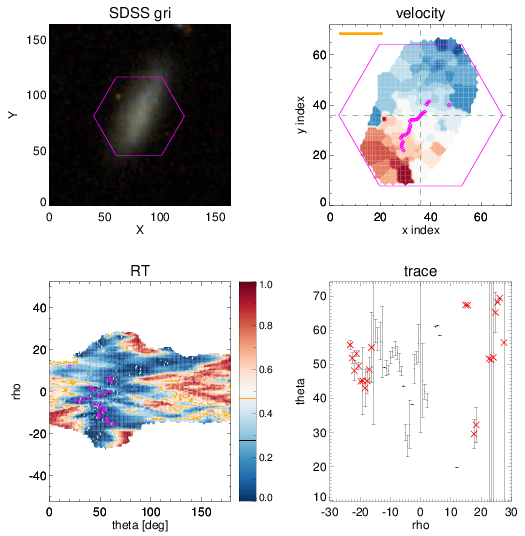
\includegraphics[width=12cm]{images/RadonPlots/RT-SNIPS-NEW/RT-CPSB-9493-12705-SNIP.png}
    \caption{Absolute Radon transform plots of the stellar velocity field of the CPSB MaNGA PLATEIFU 9493-12705. The panels show: top left - the SDSS gri image cutout; top right - the stellar velocity field. The orange coloured  bar in the upper left indicates the Radon aperture size in spaxels; bottom left - the re-scaled Radon transform. The locus of the minimum of the transform is plotted in magenta; and bottom right: the Radon trace plot. The technical details of the RT and Trace plots are described in the text.}
    \label{fig:RT-CPSB-9493-12705-SNIP}
\end{figure*}